%% josis.tex 1.4   2016-09-15    JoSIS latex template
%------------------------------------------------------------------
% Filename: josis_template.tex
%
% This file is intended as a template for typesetting articles for the
%
%                        Journal of Spatial Information Science.
%
% Please edit this template to generate your own formatted manuscripts
% for submission to JOSIS. See http://josis.org for further details.
%


%%% JOSIS checks in typesetting
%%% * All titles and sections lower case *EXCEPT short title  [ ]
%%% * Remove author postal addresses, only have geographic places and institutions [ ] 
%%% * Consistent use of Section, Figure, Table (capitalized and in full) [ ]
%%% * 10 keywords (and all lower case) [ ]
%%% * Remove all avoidable footnotes [ ]
%%% * Use double quotation marks (``'' not "" or `') [ ]
%%% * Punctuation inside quotations [ ]
%%% * E.g. and i.e. followed by comma [ ]
%%% * cf. followed by tilde [ ]
%%% * Itemize and enumerate correctly punctuated [e.g., "1. x, 2. y, and 3. x." ]
%%% * And/or lists using American English punctuation (e.g., "x, y, and z") [ ] 
%%% * Bibliography (e.g., en-dashes for number ranges, consistent "Proc.~" for Proceedings of..., etc.) []
%%% * Acknowledgment style use section* [ ] 
%%% * et al. no italics, but with dot  [ ] 
%%% * All captions end with full stop  [ ] 
%%% * Table captions under, not over table  [ ]
%%% * Adjust urls with burlalt [ ] 
%%% * Check correct use of hyphens, emdashes, endashes  [ ]
%%% * Perform spell check  [ ] 

%%% JOSIS checks directly before publication 
%%% Check DOI, page numbers on article and web site. [ ]
%%% Update web site with final title, abstract, keywords. [ ] 
%%% Build with distiller for DOI links. [ ]


% Required documentclass definition for JOSIS
\documentclass{josis}
\usepackage{hyperref}
\usepackage[hyphenbreaks]{breakurl}
\usepackage{booktabs}
\usepackage{stmaryrd}
\usepackage[T1]{fontenc}
\usepackage{cite}

% Suggested packages for algorithm formatting
\usepackage{algorithm}
%\usepackage{algorithmic}
\usepackage{algpseudocode}


\usepackage[table]{xcolor}
\usepackage{amssymb,amsmath}



\newcommand{\M}[1]{{\color{blue}\textbf{Martijn: #1}}}
\newcommand{\R}[1]{{\color{red}\textbf{Robin: #1}}}

\renewcommand{\topfraction}{0.9} 
\renewcommand{\textfraction}{0.1}

% Page setup and overhangs
\sloppy
\widowpenalty=10000
\clubpenalty=10000
\hyphenpenalty=75

% Article details for accepted manuscripts will be added by editorial staff
% Omit year if article in press
% Omit number if article under review
\josisdetails{%
   number=N, year=YYYY, firstpage=xx, lastpage=yy, 
  doi={10.5311/JOSIS.YYYY.II.NNN},
   received={December 24, 2015}, 
   returned={February 25, 2016},
   revised={July 13, 2016},
   accepted={September 5, 2016}, }

\newcommand{\mydoi}[1]{\href{http://dx.doi.org/#1}{doi:\protect\detokenize{#1}}}

%\renewcommand{\UrlLeft}{http:\sslash}
%\DeclareUrlCommand\myurl{\def\UrlLeft{}\def\UrlRight{}%
%\urlstyle{tt}}

\urlstyle{rm}
\makeatletter
% Inspired by http://anti.teamidiot.de/nei/2009/09/latex_url_slash_spacingkerning/
% but slightly less kern and shorter underscore
\let\UrlSpecialsOld\UrlSpecials
\def\UrlSpecials{\UrlSpecialsOld\do\/{\Url@slash}\do\_{\Url@underscore}}%
\def\Url@slash{\@ifnextchar/{\kern-.11em\mathchar47\kern-.2em}%
    {\kern-.0em\mathchar47\kern-.08em\penalty\UrlBigBreakPenalty}}
\def\Url@underscore{\nfss@text{\leavevmode \kern.06em\vbox{\hrule\@width.3em}}}
\makeatother

\hypersetup{
colorlinks=true,
linkcolor=black,
citecolor=black,
urlcolor=black
} 


% Our own definitions
\graphicspath{{figures/}} % where to search for the images




% Add the running author and running title information
\runningauthor{\begin{minipage}{.9\textwidth}\centering Author1, Author2\end{minipage}}
\runningtitle{ClockBoard}

% Document begins
\begin{document}
%\setcounter{page}{33}


% Insert your own title
\title{ClockBoard: a zoning system for urban analysis}

% Insert your manuscipts authors, affiliations, and addresses
\author{Robin Lovelace}\affil{Institute for Transport Studies, Leeds, University of Leeds, UK}
\author{Martijn Tennekes}\affil{Department of Methodology, Statistics Netherlands, The Netherlands}

\maketitle

% Add 5-10 keywords for every submission
\keywords{zoning, areal data, geographic data}

% Add a short abstract of 150-250 words
\begin{abstract}
Zones are the building blocks of urban analysis.
Fields ranging from demographics to transport planning routinely use zones --- spatially contiguous areal units that break-up continuous space into discrete chunks --- as the foundation for diverse analysis techniques.
Key methods such as origin-destination analysis and choropleth mapping rely on zones with appropriate sizes, shapes and coverage.
However, existing zoning systems are sub-optimal in many urban analysis contexts, for three main reasons:
1) administrative zoning systems are often based on somewhat arbitrary factors;
2) evidence-based zoning systems are often highly variable in size and shape, reducing their utility for inter-city comparison; and
%3) in many areas, especially in low income nations, high resolution zoning systems of the type required for many urban analysis tasks are simply unavailable.
3) the resolution of existing zoning systems is often too low for certain urban analysis, especially in low income nations.
To tackle these three key issues we developed a flexible, open and scalable solution: the ClockBoard zoning system.
ClockBoard consists of 12 segments divided by concentric rings of increasing distance, creating a consistent visual frame of reference for cities that is reminiscent of a clock and a dartboard.
This paper outlines the design, potential uses and merits of the ClockBoard zoning system and discusses future avenues for research and development of new zoning systems based on the experience.
\end{abstract}

% Your main text begins here. 
\section{Introduction}

Zoning systems have long been used for practical purposes.
They have been integral to land ownership, rents and urban policies for centuries, forming the basis of a range of social and economic practices.
Historical examples highlighting the importance of zone layouts include 'tithe maps' determining land ownership and taxes in 18th Century England \cite{bryant_worcestershire_2007} and legally defined urban land use zones to tame chaotic urban growth expansion in the exploding US cities in the early 1900s \cite{baker_zoning_1925}.

In the 19th Century, zoning systems became known for political reasons, with 'gerrymandering' entering public discourse and academic research following Elbridge Gerry's apparent attempt to gain political advantage by creating an electoral district in an odd shape that was said to resemble a salamander (hence the term's name) in 1812  \cite{orr_persistence_1969}.
The gerrymandering problem has since been the topic of countless academic papers.

%The problem, when described in mathematical terms, can be analysed quantitatively and even optimised:
%"$n$ units are grouped into $k$ zones such that some cost function is optimized, subject to constraints on the topology of the zones" \cite{chou_taming_2006}.
The gerrymandering problem (in itself is a manifestation of the modifiable area unit problem) can be described as a mathematical optimization problem: "$n$ units are grouped into $k$ zones such that some cost function is optimized, subject to constraints on the topology of the zones" \cite{chou_taming_2006}.
%This, in fact, is a concise definition of the broader "zoning problem" of which gerrymandering is one consequence (which in itself is a manifestation of the modifiable area unit problem), that starts from the assumption that zones are to be composed of one or more basic statistical units (BSUs).
%This, in fact, is a concise definition of the broader "zoning problem" of which gerrymandering is one consequence (which in itself is a manifestation of the modifiable area unit problem), that starts from the assumption that zones are to be composed of one or more basic statistical units (BSUs).
In fact, this problem is concise definition of the broader "zoning problem" that starts from the assumption that zones are to be composed of one or more basic statistical units (BSUs).
Although the range of outcomes is a finite combinatorial optimisation problem (which combination of BSU-zone aggregations satisfy/optimise some pre-determined criteria) the problem is still hard:
"there are a tremendously large number of alternative partitions, a similar number of different results, and only a slightly smaller number of different interpretations" \cite{openshaw_optimal_1977}.

The problem that we tackle in this paper is different, however: it is the division of geographic space into zones \textbf{starting from a blank slate}, without reference to pre-existing areal units.
The focus of much preceding zoning research on BSU partitioning can be explained by the fact that much geographic data available to academics comes in 'pre-packaged' small areas and because creating zones from nothing is a harder problem.
We disagree with the statement that "existence of individual or non-spatially aggregated data is rare in geography" \cite{openshaw_optimal_1977}, pointing to car crashes, shop locations, species identification data and dozens of other phenomena that can be understood as 'point pattern processes'.
And with advances in computer hardware and software, the 'starting from scratch' approach to zoning system is more feasible.

A number of approaches have tackled the question of how to best divide up geographical space for analysis and visualisation purposes, with a variety of applications.
Functional zone classification is common in the field of remote sensing and associated sub-fields involved in analysing and classifying raster datasets \cite{ciglic_evaluating_2019} \cite{hesselbarth_landscapemetrics_2019}.
While such pixel-based approaches can yield complex and flexible results (depending on the geographic resolution of the input data), they are still constrained by the building blocks of the pixels, which can be seen as a particular type of areal unit, a uniformly sized and shaped BSU.

In this paper we are interested in the division of \emph{continuous space} into completely new areal systems.
This has been done using contour lines to represent lines of equal height, and the concept's generalisation to lines of equal journey time from locations (isochrones) \cite{long_modeling_2018}, population density (isopleths) \cite{lin_cartographic_2017} and model parameters which continuous geographical space \cite{paez_exploring_2006}.
The boundaries created by these various `iso' maps are `procedurally generated' areal units of the type that this paper focuses, but their variability and often irregular shapes make them impractical for many types of urban analysis.

Procedural generation, which involves the generation of data through a repeated and sometimes randomised computational process has long been used to represent physical phenomena \cite{onrust_ecologically_2017}.
The approach has been used to generate spatial entities including roads \cite{galin_procedural_2010}, indoor layouts of buildings \cite{anderson_augmented_2018} and urban layouts \cite{mustafa_procedural_2020}.
Algorithms have also been developed to place linear features on a map, as illustrated by an algorithm that optimizes the placement of overlapping linear features for cartographic visualisation \cite{teulade-denantes_routes_2015}.
However, no previous research has demonstrated the creation of zoning systems specifically for the purposes of urban analysis.

New visualisation techniques are needed to represent new (or newly quantifiable) concepts and emerging datasets (such as OpenStreetMap) in urban analysis analysis .
The visualisation of direction has been driven by new navigational requirements and datasets, with circular compasses and displays common in land and sea navigational systems since the mid 1900s \cite{honick_pictorial_1967}.
Circular visualisation techniques, in the form of rose diagrams, were used in a more recent study to indicate the most common road directions relative to North \cite{boeing_spatial_2021}.
The resulting visualisations are attractive and easy to interpret, but are not geographical, in the sense that they cannot meaningfully be overlaid on mapped data.
The approach we present in this paper is more closely analogous to `grid sample' approaches used in ecological and population research \cite{hirzel_which_2002} .
Historically, environmental researchers have used rectangular (and usually square) grids to divide up space and decide sampling strategies.
Limitations associated with this simplistic strategy have been documented since at least the 1960s, with a prominent paper on geographic sampling strategies outlining advantages and disadvantages of simple random, systematic and stratified sampling techniques in 1967 \cite{holmes_problems_1967}.
Starting with data at the level of raster grid cells and BSUs, a related approach is to sample from within available `pixels' to generate a representative sample \cite{thomson_gridsample_2017}.


Unlike BSU based zoning systems, grid sampling strategies require no prior zones.
Unlike `procedurally generated' areas, grid-based strategies generate areal units of consistent sizes and shapes.
However, grid-based strategies are limited in their applicability to urban research because they seldom generate geographically contiguous results and do not account for the strong tendency of human settlements to have a (more-or-less clearly demarcated) central location with higher levels of activity.

Pre-existing zoning systems are often based on administrative regions. Although those zoning systems are usually in line with the hierarchical organization structure of governmental organizations, and therefore may work well for policy making, there are a couple of downsides to using such zoning systems. First of all, since a city and its politics change over time, the administrative regions often change accordingly. This make it harder to do time series analysis. Since the administrative regions have heterogeneous characteristics, for instance population size, area size, proximity to the city centre, comparing different administrative regions within a city is not straightforward. Moreover, comparing administrative regions across cities is even more challenging since average scale of an administrative region may vary a lot across cities.

Grid tiles are popular in spatial statistics for a number of reasons. Most importantly the tiles have a constant area size, which makes comparably possible. Moreover, the grid tiles will not change over time like administrative regions. However, one downside is that a grid requires a coordinate reference system (CRS), enforcing (approximately) equal area size. For continents or large countries, a CRS is always a compromise. Therefore, the areas of the tiles may vary, or the shape of the tiles may be sheared or warped.

Another downside from a statistical point of view is that population densities are not uniform within a urban area, but concentrated around a centre. As a consequence, high resolution statistics is preferable in the dense areas, i.e. the centre, and lower resolution statistics in other parts of the city. That is the reason why administrative regions are often smaller in dense areas.

The approach presented in this paper aims to minimise input data requirements, generate consistent zones comparable between widely varying urban systems, and provide geographically contiguous areal units.
%The problem that we address in this paper, in other words, is
%From a research perspective, the way in which ... \cite{openshaw_optimal_1977}
% \subsection{Limitations of pre-existing zoning systems}
%\subsection{The rational for new zoning systems}
%\M{Work this out} (worked out)
The motivations for generating a new zoning system and use cases envisioned include:

\begin{itemize}
    \item Locating cities. Automated zoning systems based on a clear centrepoint can support map interpretation by making it immediately clear where the city centre is, and what the scale of the city is. 
    \item Reference system of everyday live. The zone name contains information about the distance to the center as well as the cardinal direction. E.g "I live in C12 and work in B3." or "The train station is in the center and our hotel is in B7". Moreover, the zones indicate whether walking and cycling is a feasibly option regarding the distance.
    \item Aggregation for descriptive statistics / comparability over cities. By using the zoning system to aggregate statistics (e.g. on population density, air quality, bicycle use, number of dwellings), cities can easily be compared to each other.
    \item Modelling urban cities. The zoning system can be used to model urban mobility.
\end{itemize}

The paper is structured as follows.
The next section outlines the approach, which requires only 2 inputs: the coordinates of the central place in the urban system under investigation, and the minimum radius from that central point that the zoning system should extend.
Section 3 describes a number of potential applications, ranging from rudimentary navigation and location identification to mobility analysis.
Finally, in Section 4, we discuss limitations of the approach and possible directions of research and development to generate additional zoning systems for urban analysis.

\section{The ClockBoard zoning system}

% This section explains what the ClockBoard is

The ClockBoard zoning system tackles the various issues outlined above based on the following desirable criteria for zoning systems from an urban analysis:

- Intuitive naming system for the individual zones within
- Easy to visualise without too many (500+) or too few (less than 10) individual zones
- Zone sizes decrease with distance from the city centre, highlighting the relative importance and population density towards the centre of many settlements
- Can represent a wide range of cities and urban forms ranging from extensive cities such as Mexico City to compact cities such as Hong Kong

- It's a specific implementation of a general concept
- 

\subsection{Annuli distances}

The radius of each annuli in the zoning system can be incremented by a fixed amount, as shown in previous figures. %Todo: add figures
In cases where high geographic resolution is important near the centre of the study region, such as when designing transport systems into the central zone of a city planning, increasing distances between each radius may be desirable.
We experimented with various ways of incrementing the annuli width and suggest linear increases in width as a sensible default for a simple zoning system.
This linear growth leads to distances between each annuli boundary increasing in line with the steps in the \href{https://en.wikipedia.org/wiki/Triangular_number}{triangular number sequence} \cite{ross_dicuil_2019}.

% latex table generated in R 4.0.3 by xtable 1.8-4 package
% Fri Feb 19 15:32:48 2021
\begin{table}
\centering
\begin{tabular}{rrrr}
  \hline
 & Number of rings & Diameter across (km) & Area (sq km) \\ 
  \hline
1 &   1 & 2 & 3.14 \\ 
  2 &   2 & 6 & 28.27 \\ 
  3 &   3 & 12 & 113.10 \\ 
  4 &   4 & 20 & 314.16 \\ 
  5 &   5 & 30 & 706.86 \\ 
  6 &   6 & 42 & 1385.44 \\ 
  7 &   7 & 56 & 2463.01 \\ 
  8 &   8 & 72 & 4071.50 \\ 
  9 &   9 & 90 & 6361.73 \\ 
   \hline
\end{tabular}
\end{table}


\subsection{Number of segments}

What it looks like with 4 segments.

\subsection{City extents}

\section{Applications}

\subsection{Navigation and location}


\subsection{Exploring city scale data}
univariate description

- Population density in London
- Social (e.g. religion) and demographic distributions

\subsection{Inter-city statistical comparison}

\begin{figure}[tbh]
\centering
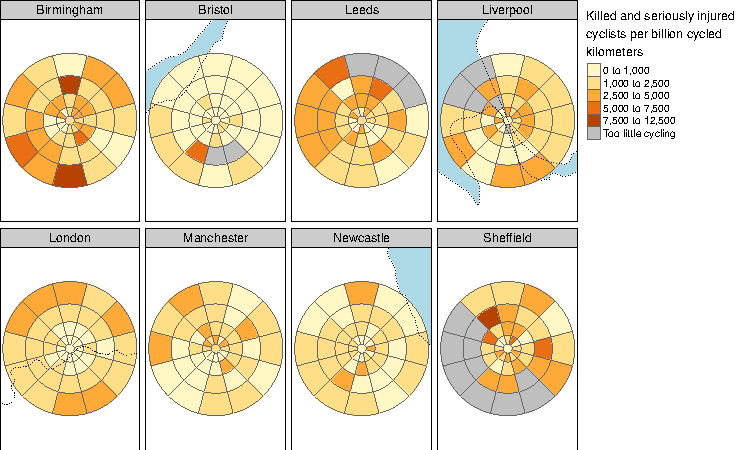
\includegraphics[width=\textwidth]{cycling_accidents.pdf}
\caption{Cycling accidents compared between eight cities.}\label{fig:cyclAccidents}
\end{figure}

\subsection{Mobility analysis}

% OD data aggregated to ClockBoard zones

\section{Discussion and conclusions}


\subsection{Limitations}

Pros:

\begin{itemize}
\item Most cities have a radial plan around a central area, which is often a historic centre or a central business area. Typically, this centre is not only the geographic centre, but also the busiest area in terms of daytime population. Often the main nodes in the urban transport network are also located in or near the city centre. Note that many cities already consist of concentric rings, separated by a ring road. (See also \url{https://en.wikipedia.org/wiki/City_centre} which describes the centre as the heart of the city)
\end{itemize}

Cons:

\begin{itemize}
\item Some cities have two or more centres. Many cities have a central business discrict or financial discrict which not always coinsides with the historic city centre.
\item In urban areas with nearby cities, it may not always be clear where one cities ends and another begins. Also, small cities may be located within the metropolitan area of a larger city (e.g. the Dutch cities The Hague/Delft)
\end{itemize}

\bibliographystyle{josisacm}
\bibliography{references}

\appendix
\section{World cities}

\begin{figure}[tbh]
\centering
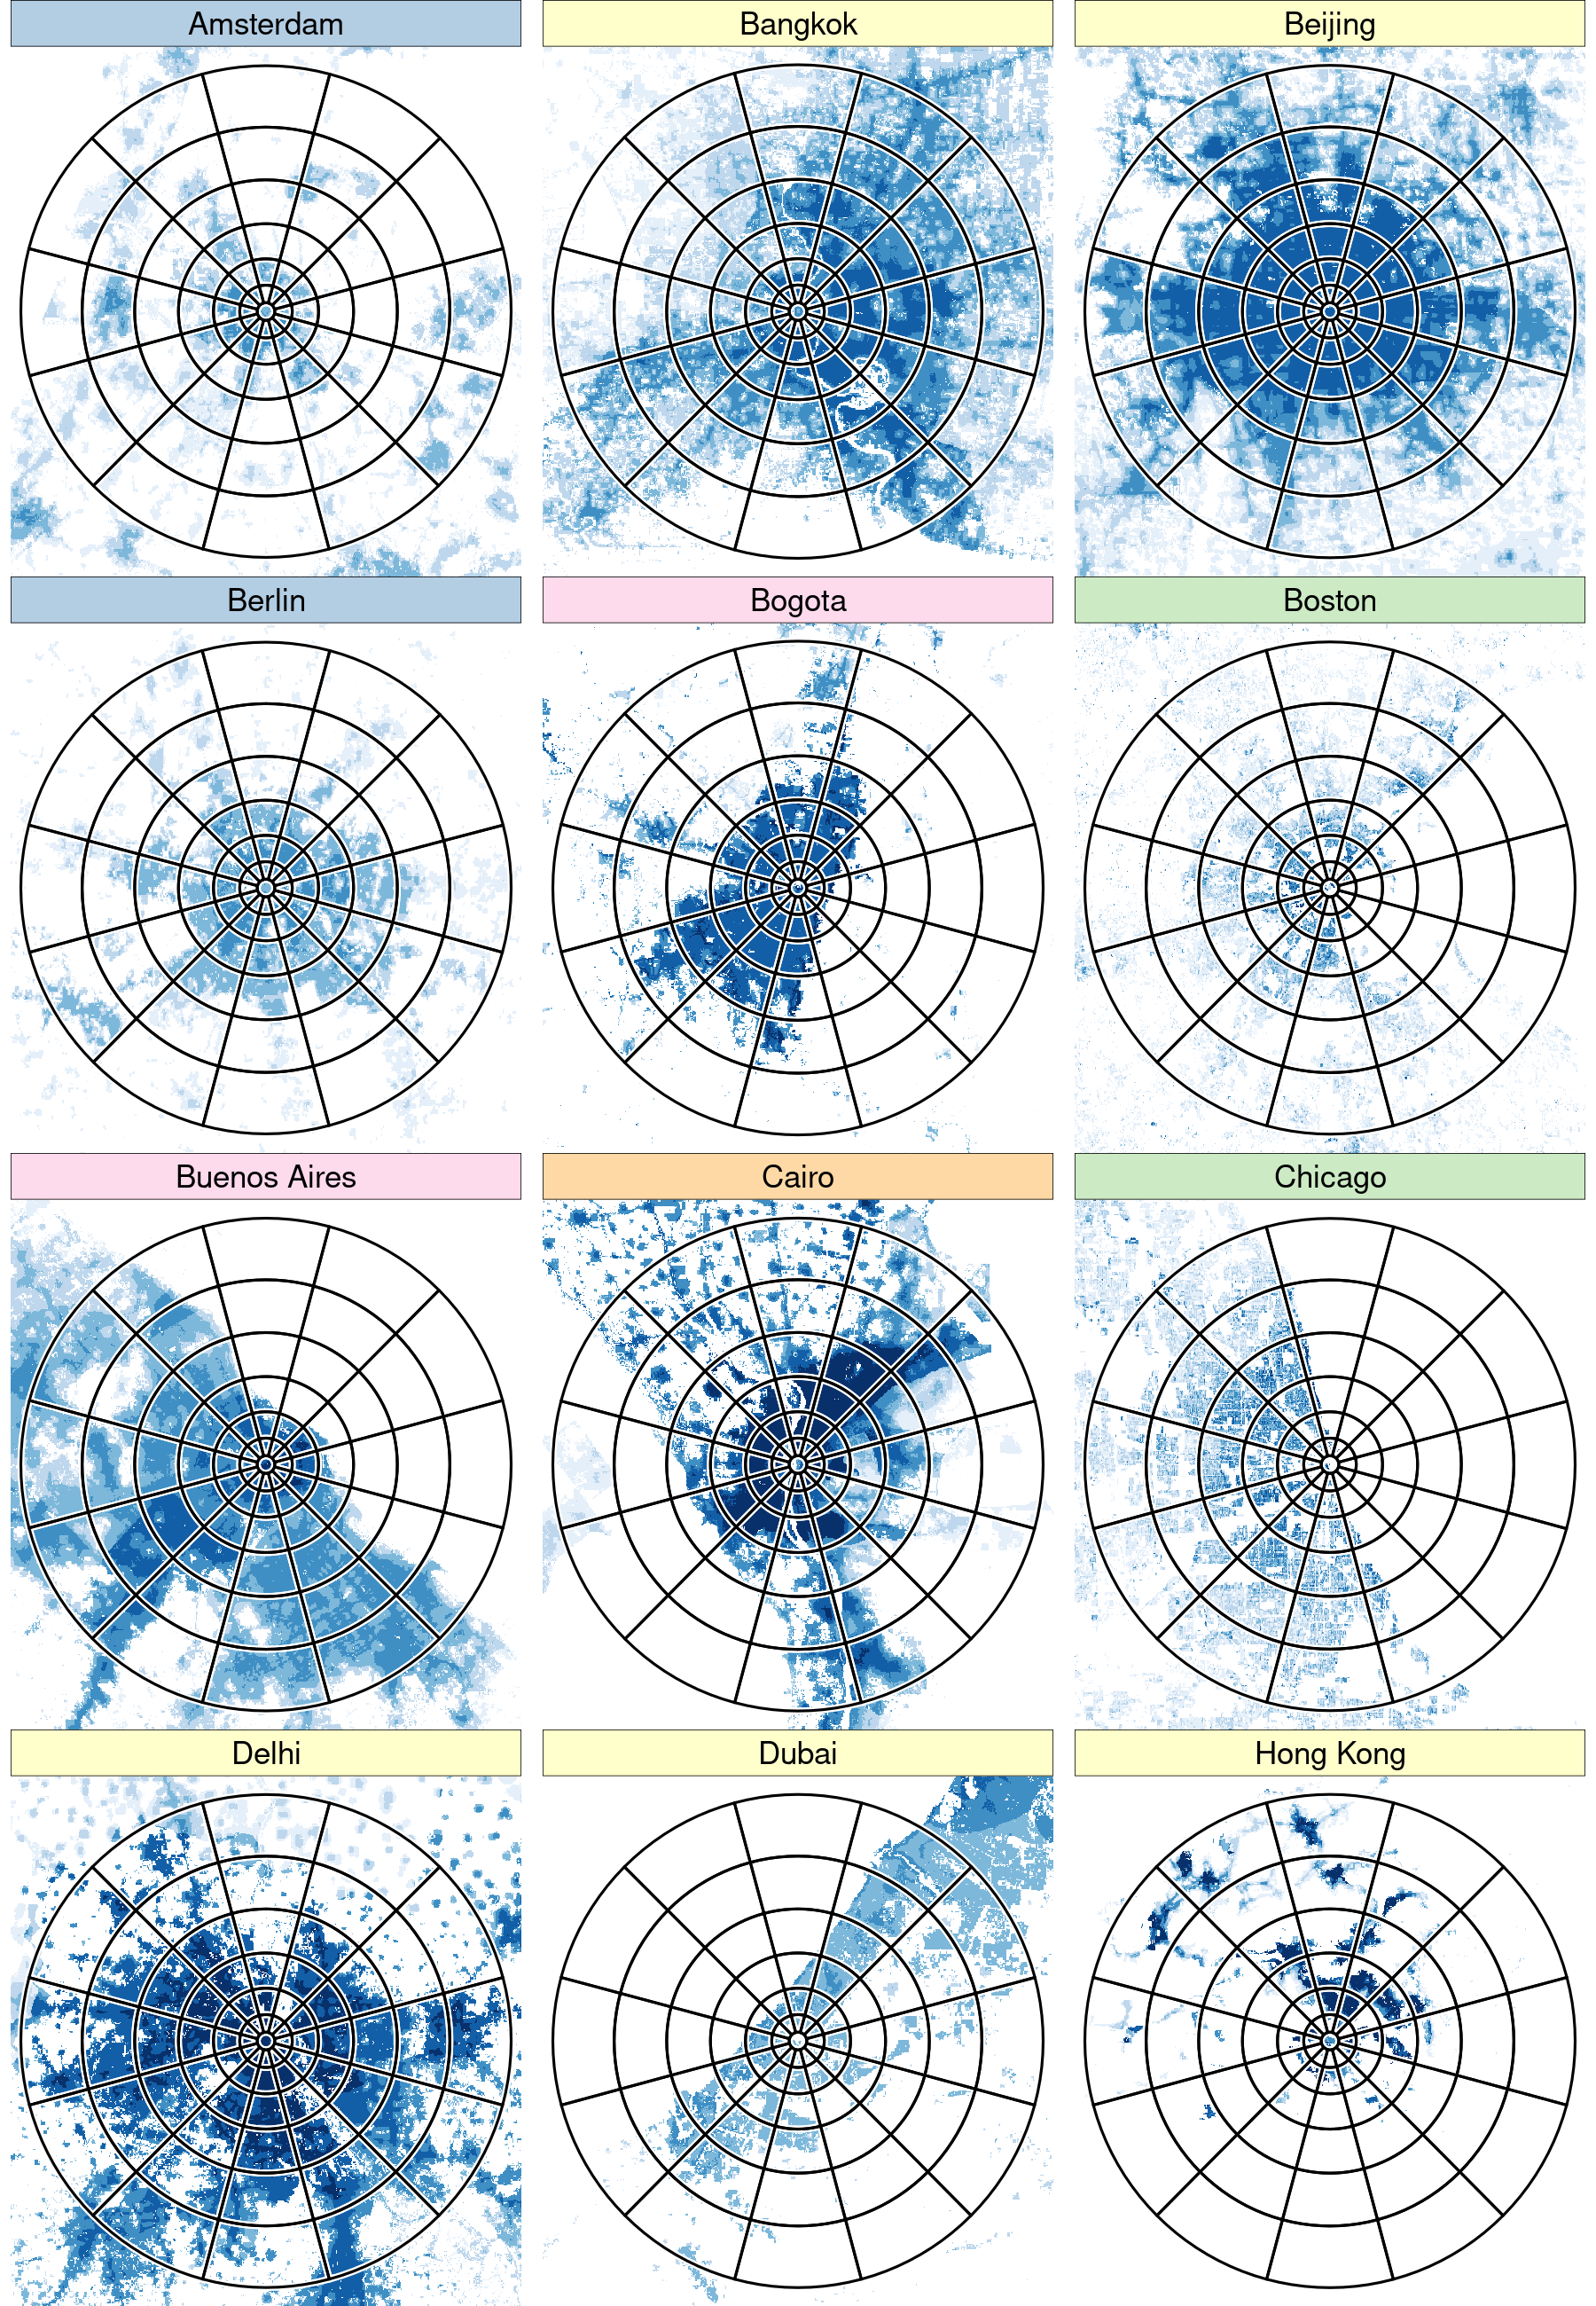
\includegraphics[width=\textwidth]{cities_page1.png}
\caption{ClockBoard for 36 cities, with population density shown in blue, and continent shown in the header color.}\label{fig:cities1}
\end{figure}

\begin{figure}[tbh]
\centering
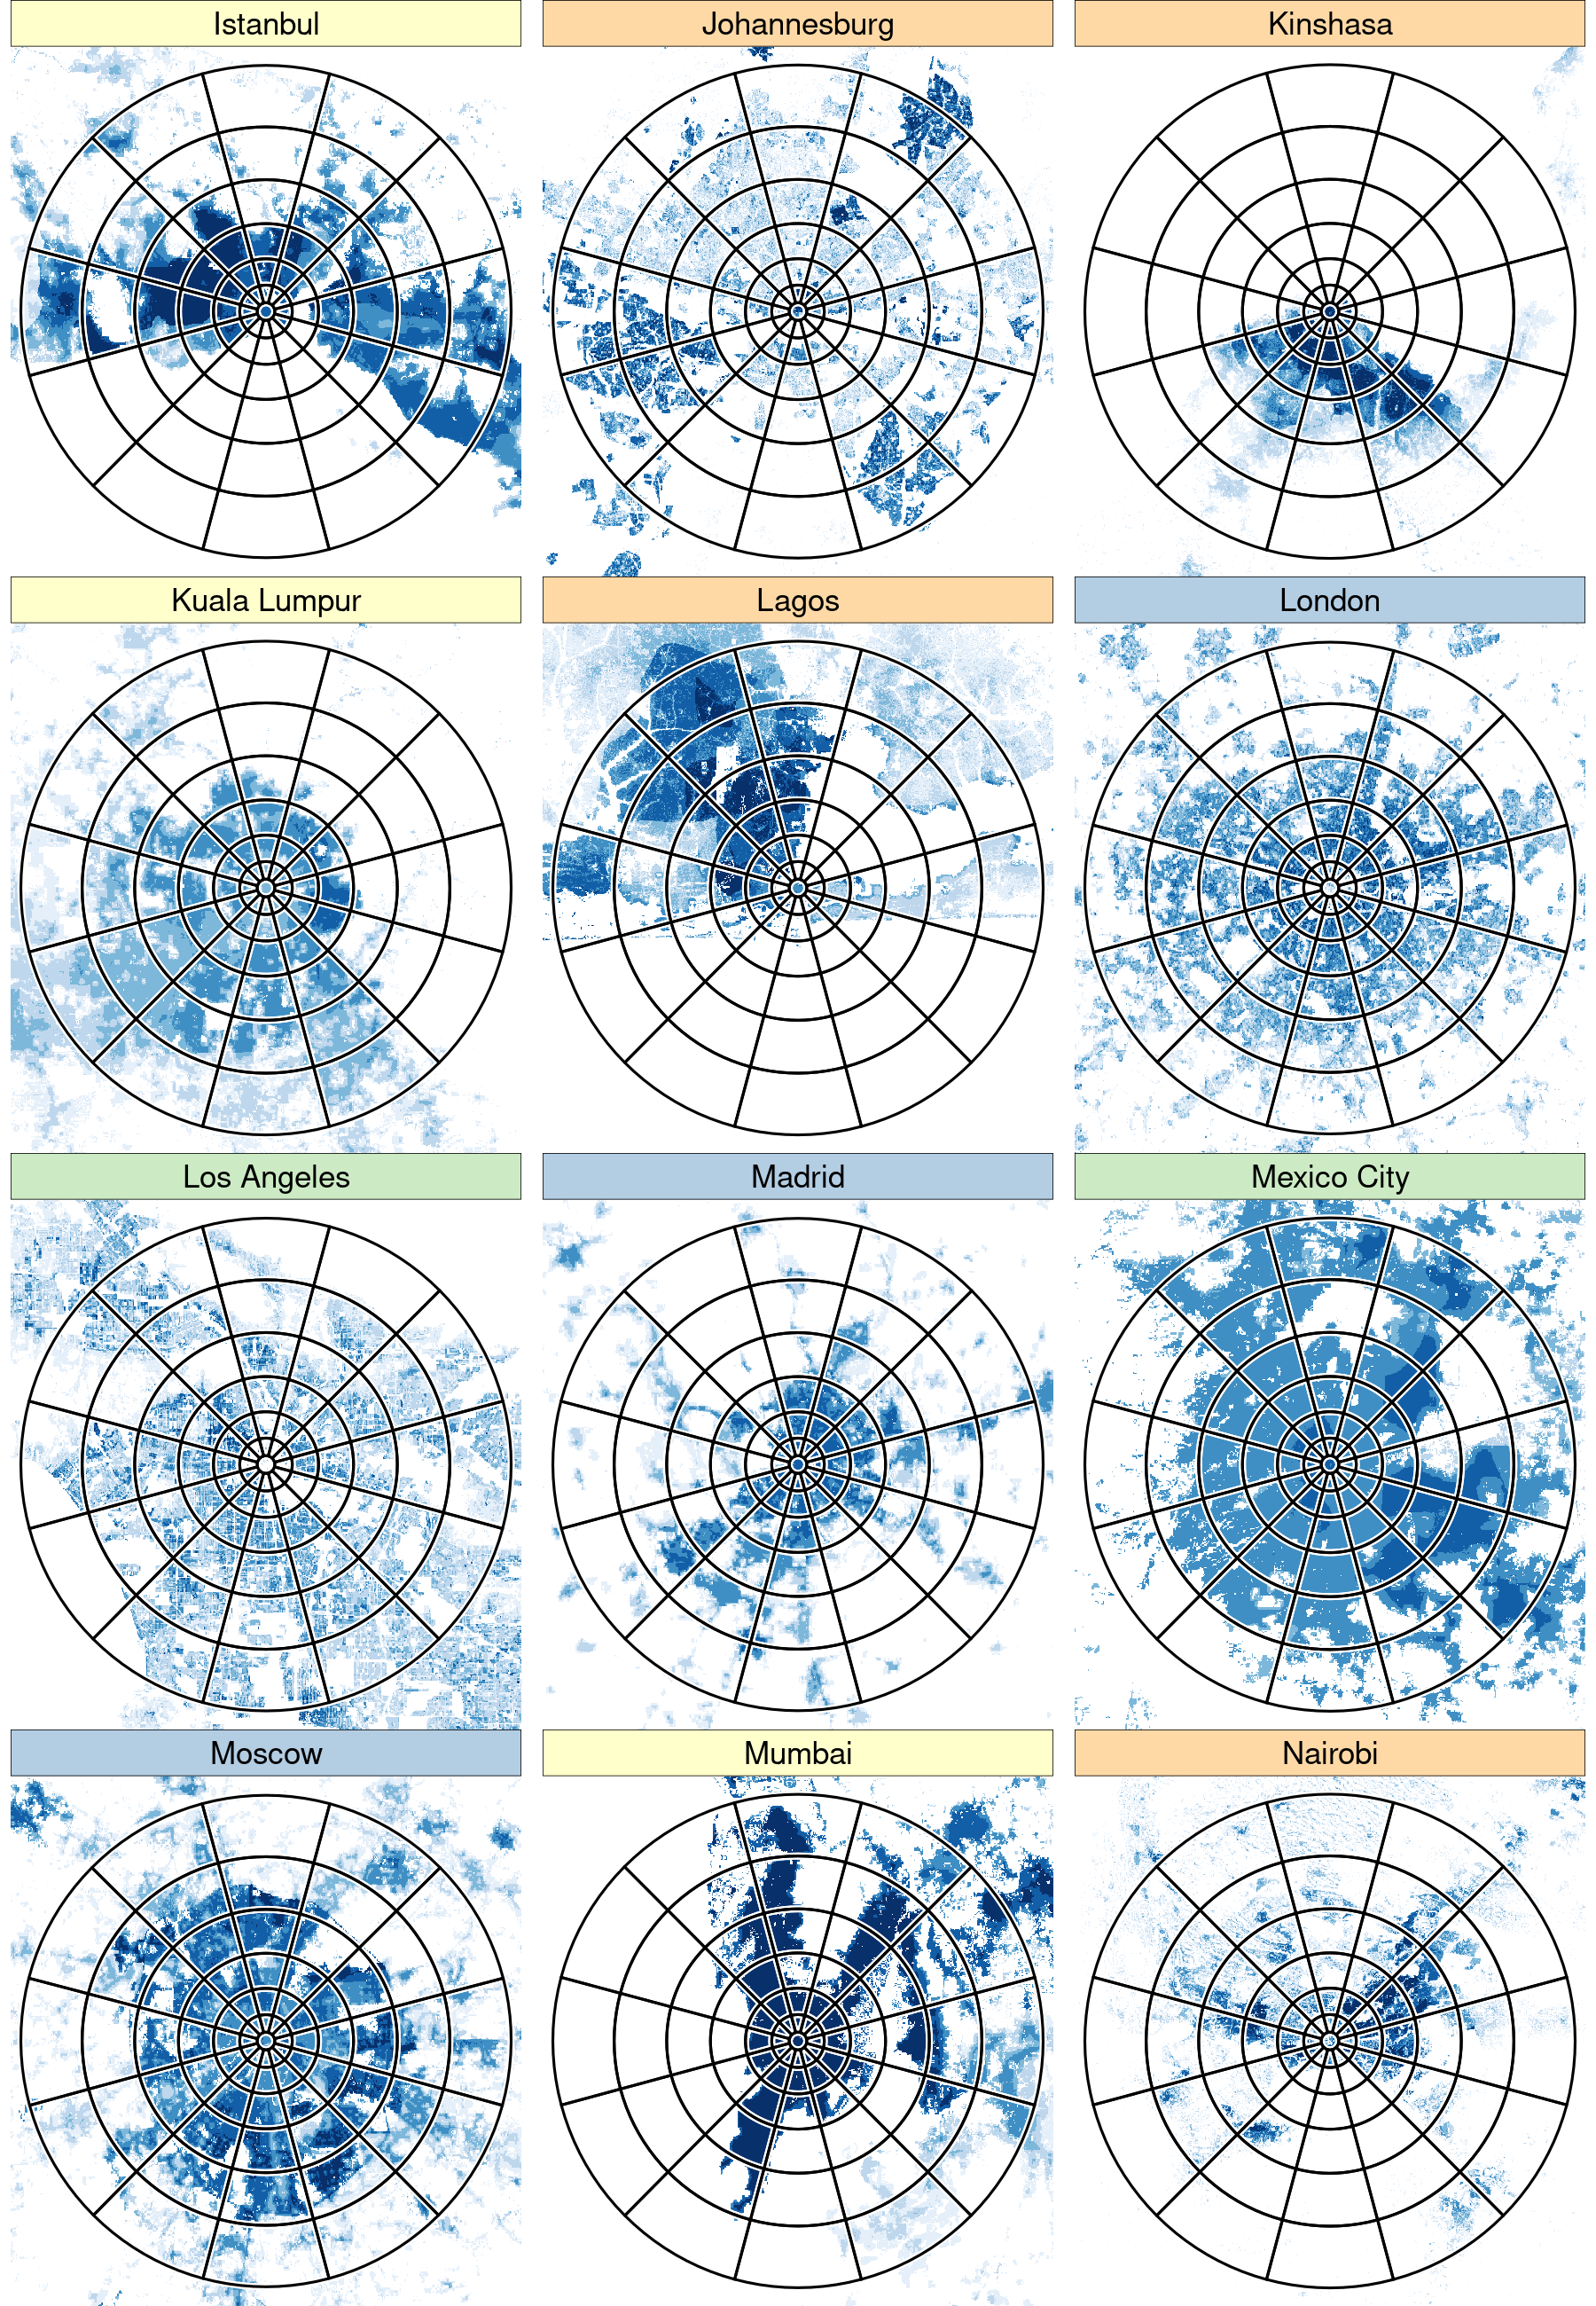
\includegraphics[width=\textwidth]{cities_page2.png}
\caption{(continued)}\label{fig:cities2}
\end{figure}

\begin{figure}[tbh]
\centering
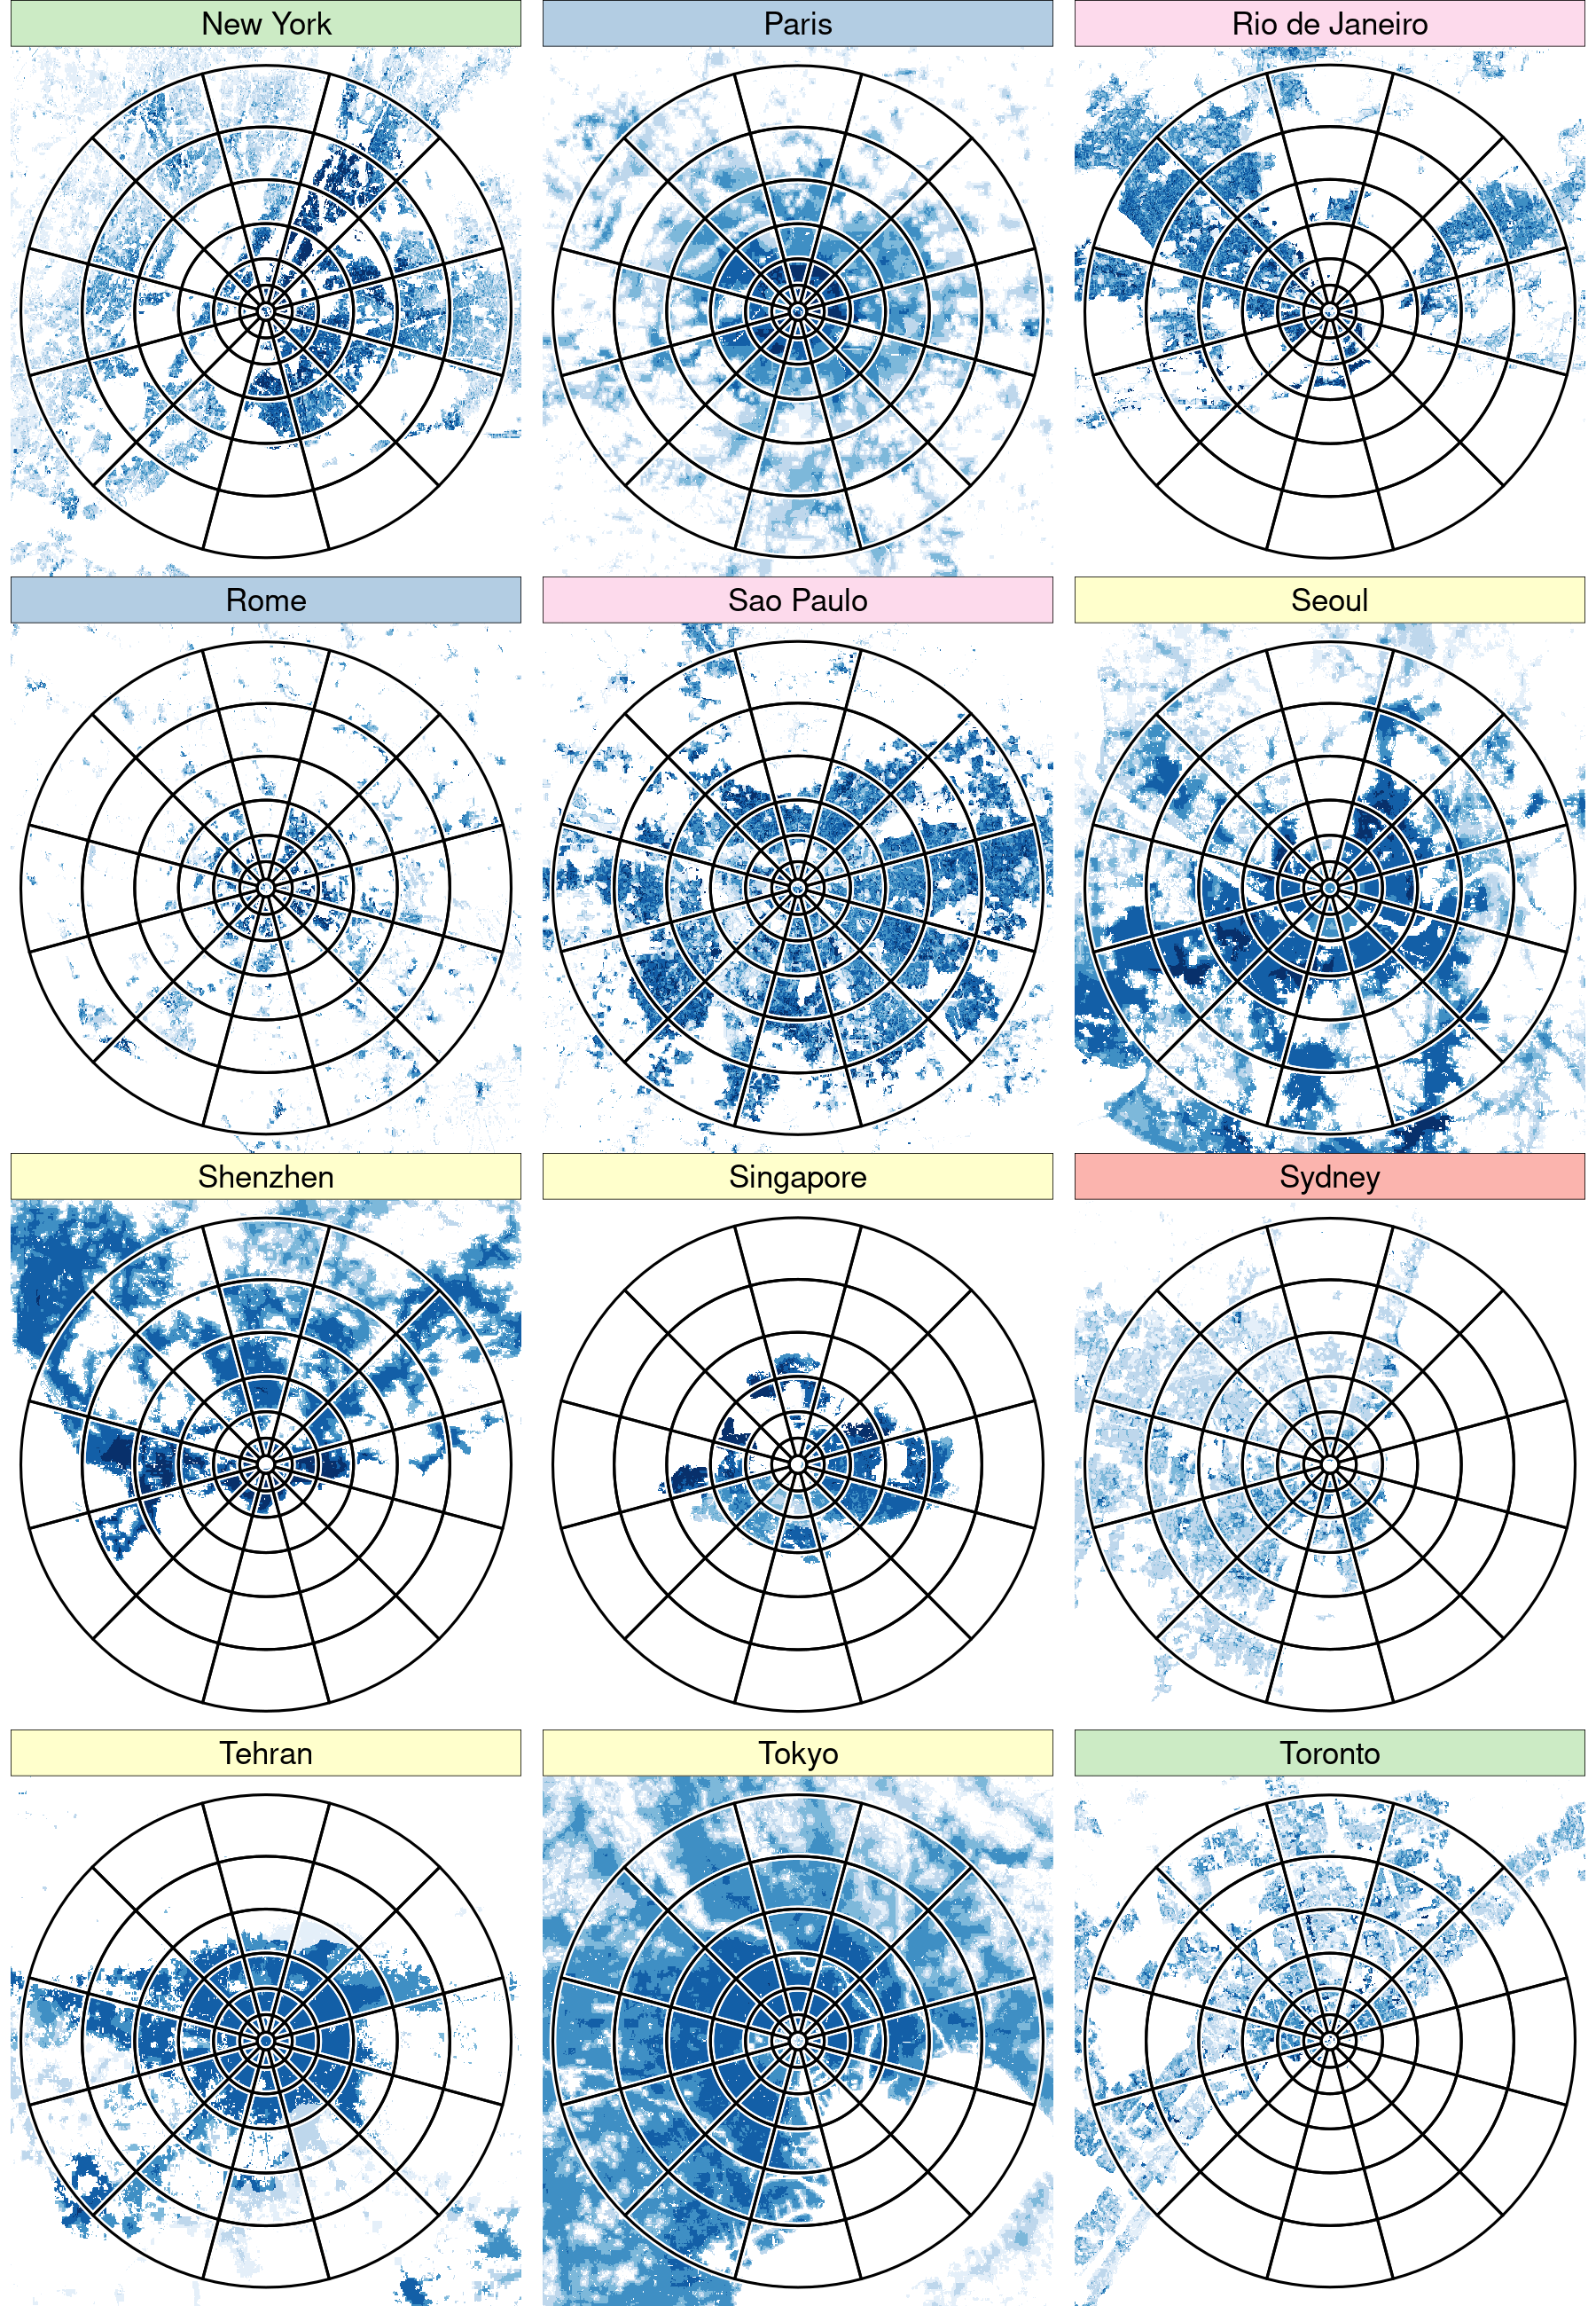
\includegraphics[width=\textwidth]{cities_page3.png}
\caption{(continued)}\label{fig:cities3}
\end{figure}

\end{document}